	%-=-=-=-=-=-=-=-=-=-=-=-=-=-=-=-=-=-=-=-=-=-=-=-=
%
%        LOADING DOCUMENT
%
%-=-=-=-=-=-=-=-=-=-=-=-=-=-=-=-=-=-=-=-=-=-=-=-=

\documentclass[newPxFont,pagenumber]{beamer}
\usetheme{sthlm}
%\usecolortheme{sthlmv42}

%-=-=-=-=-=-=-=-=-=-=-=-=-=-=-=-=-=-=-=-=-=-=-=-=
%        LOADING PACKAGES
%-=-=-=-=-=-=-=-=-=-=-=-=-=-=-=-=-=-=-=-=-=-=-=-=
\usepackage[utf8]{inputenc}
\usepackage[frenchb]{babel}
\usepackage[normalem]{ulem}
\usepackage{caption}
\captionsetup{font=scriptsize}
%\usepackage[font=footnotesize]{subcaption}
% in preamble
\usepackage{chronology}
\usepackage{pgf}
\usepackage{tikz}
\usetikzlibrary{arrows,automata}
\usepackage{array,multirow}
\usepackage{nameref}
\makeatletter
\newcommand*{\currentname}{\@currentlabelname}
\makeatother

\graphicspath{ {fig/} }

\usepackage[linesnumbered,ruled,vlined]{algorithm2e}
% add page number
%\usepackage[defaultsans]{cantarell}

\newcommand{\p}{\mathbb{P}}

\setbeamerfont{title}{series=\upshape}
\setbeamertemplate{footline}{\hfill\footnotesize\insertframenumber\hskip3pt\null\vskip3pt}

\newcommand{\argmax}{\mathop{\mathrm{argmax}}\limits}
\renewcommand{\max}{\mathop{\mathrm{max}}\limits}

\renewcommand{\event}[3][e]{%
  \pgfmathsetlength\xstop{(#2-\theyearstart)*\unit}%
  \ifx #1e%
    \draw[fill=black,draw=none,opacity=0.5]%
      (\xstop, 0) circle (.2\unit)%
      node[opacity=1,rotate=45,right=.2\unit] {#3};%
  \else%
    \pgfmathsetlength\xstart{(#1-\theyearstart)*\unit}%
    \draw[fill=black,draw=none,opacity=0.5,rounded corners=.1\unit]%
      (\xstart,-.1\unit) rectangle%
      node[opacity=1,rotate=45,right=.2\unit] {#3} (\xstop,.1\unit);%
  \fi}%

\addto\captionsfrench{%
\renewcommand{\figurename}{\scriptsize {\scshape Figure}}
\renewcommand{\tablename}{\scriptsize {\scshape Table}}
}

%-=-=-=-=-=-=-=-=-=-=-=-=-=-=-=-=-=-=-=-=-=-=-=-=
%        BEAMER OPTIONS
%-=-=-=-=-=-=-=-=-=-=-=-=-=-=-=-=-=-=-=-=-=-=-=-=

%\setbeameroption{show notes}

%-=-=-=-=-=-=-=-=-=-=-=-=-=-=-=-=-=-=-=-=-=-=-=-=
%
%	PRESENTATION INFORMATION
%
%-=-=-=-=-=-=-=-=-=-=-=-=-=-=-=-=-=-=-=-=-=-=-=-=

\title{\vspace{0.4cm}\normalsize Analyse sémantique d’un corpus exhaustif de décisions jurisprudentielles pour l'élaboration d’un modèle prédictif du risque judiciaire     }
\subtitle{
%\scriptsize Comité de suivi individuel -- \textit{12 juillet 2017}
}
%\date{\small{\jobname}}
\date{\scriptsize Début de thèse: 15 Décembre 2015}
\author{
%\normalsize Gildas Tagny Ngompé
}
\institute{\scriptsize 
\textbf{Doctorant:} Gildas Tagny Ngompé

\textbf{Direction de thèse:} \begin{itemize}
\item Jacky Montmain (École des mines d'Alès, LGI2P)
\item Stéphane Mussard (Université de Nîmes, CHROME)
\end{itemize}
\textbf{Encadrement de proximité:} \begin{itemize}
\item Sébastien Harispe (Ecole des Mines d'Alès, LGI2P)
\item Guillaume Zambrano (Université de Nîmes, CHROME)
\end{itemize}}

\hypersetup{
pdfauthor = {\author{}: tagnyngompe@gmail.com},
pdfsubject = {},
pdfkeywords = {},
pdfmoddate= {D:\pdfdate},
pdfcreator = {}
}

\begin{document}
\nocite{}
%-=-=-=-=-=-=-=-=-=-=-=-=-=-=-=-=-=-=-=-=-=-=-=-=
%
%	TITLE PAGE
%
%-=-=-=-=-=-=-=-=-=-=-=-=-=-=-=-=-=-=-=-=-=-=-=-=
\begin{frame}[plain]
	\titlepage
\end{frame}
%}
%-=-=-=-=-=-=-=-=-=-=-=-=-=-=-=-=-=-=-=-=-=-=-=-=
%
%	TABLE OF CONTENTS: Plan
%
%-=-=-=-=-=-=-=-=-=-=-=-=-=-=-=-=-=-=-=-=-=-=-=-=
\section*{Plan}
\begin{frame}[c]{\currentname}
\tableofcontents[hideallsubsections]
\end{frame}

\section{Motivations et objectifs}

\begin{frame}[c]{Les juristes analysent les décisions afin d'anticiper}
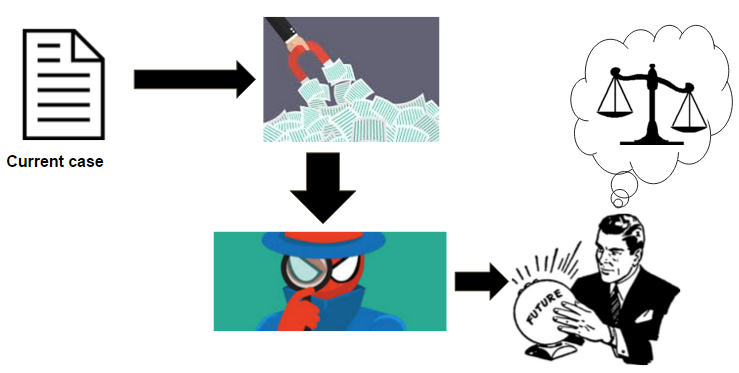
\includegraphics[width=\textwidth]{lawyerwork.png}
\end{frame}

\begin{frame}[c]{Défis: grand volume de décisions}
\textbf{Plus de 4 millions de décisions prononcées / an}
\begin{table}[!htb]
{
\footnotesize
\begin{center}
\begin{tabular}{|p{2cm}|c|c|c|c|c|}
\hline
 & \textbf{2010} & \textbf{2011} & \textbf{2012} & \textbf{2013} & \textbf{2014} \\
 \hline
 \textbf{Justice civile} & 2 673 131  & 2 654 179 & 2 647 813 & 2 761 554  & 2 618 374 \\
 \hline
\textbf{Justice pénale} & 1 173 242 & 1 180 586 & 1 251 979 & 1 303 469 & 1 203 339 \\
 \hline
 \textbf{Justice administrative} & 224 787 & 225 608 & 228 680 & 221 882 & 230 477 \\
 \hline
\end{tabular}
\textit{\tiny{Source: \url{http://www.justice.gouv.fr/budget-et-statistiques-10054/chiffres-cles-de-la-justice-10303/}}}  
\end{center}
}
\caption{Nombre de décisions prononcées en France par an}\label{decisionstats}
\end{table}
\end{frame}

\begin{frame}[t]{Défis: Recherches et analyses sémantiques difficiles}

Moteurs de recherche juridique à mots-clés 

Pas d'analyse synthétique des décisions 

%\begin{figure}
\fbox{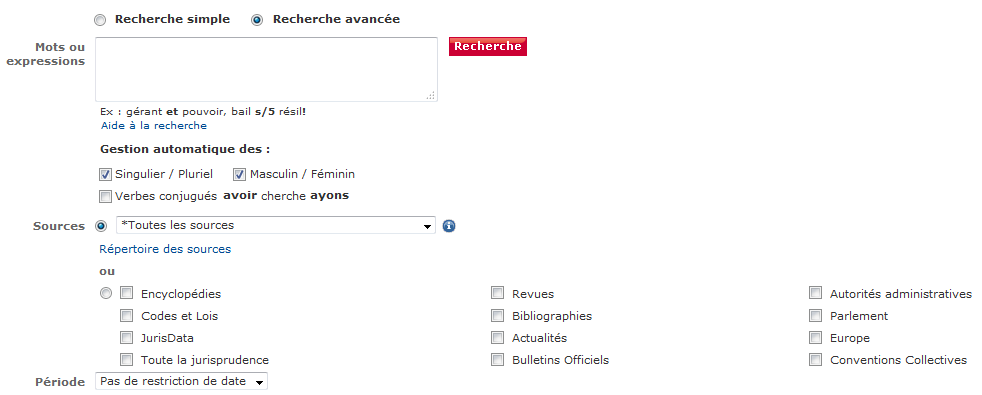
\includegraphics[width=0.9\paperwidth]{jurica.png}}

\textit{\tiny{Source: \url{LexisNexis.com}}} 
%\caption{Formulaire de recherche}
%\end{figure}
\end{frame}


\begin{frame}{Défis: Documents non-structurés et langage complexe}
\scriptsize
\begin{columns}
\begin{column}{.50\linewidth}
ARRÊT N°

R.G: 11/03924

...

{COUR D'APPEL} DE {NÎMES}

{CHAMBRE CIVILE}

{1ère Chambre A}

ARRÊT DU {20 MARS 2012}

APPELANTE:

{Madame Michéle A.} ...

assistée de la {SELARL VAJOU}, ...

INTIMES:

{Monsieur Martial B} ...

assisté de la {SCP MARION GUIZARD PATRICIA SERVAIS}, ...

COMPOSITION DE LA COUR LORS DU DÉLIBÉRÉ:

{M. Dominique BRUZY, Président}

{M. Serge BERTHET, Conseiller}

...
\end{column}
\begin{column}{.50\linewidth}
FAITS, PROCEDURE, ...

Madame Michèle A. demande:

...

- de condamner Madame JONES-B. à lui payer la somme de {2.500 euros} au titre de l'{article 700 du Code de Procédure Civile}, 

\vspace{0.4cm}

PAR CES MOTIFS, LA COUR:

...

Vu l'{article 809 du Code de Procédure Civile},

...

{Déboute Madame A. de sa demande de provision sur dommages-intérêts.}

...

Vu l'{article 700 du Code de Procédure Civile},

Condamne Madame JONES-B. à verser à Madame A. la somme de {2.500 euros}.
\end{column}
\end{columns}
\end{frame}

\begin{frame}{Notre projet: Automatiser la structuration et l'analyse}
\centering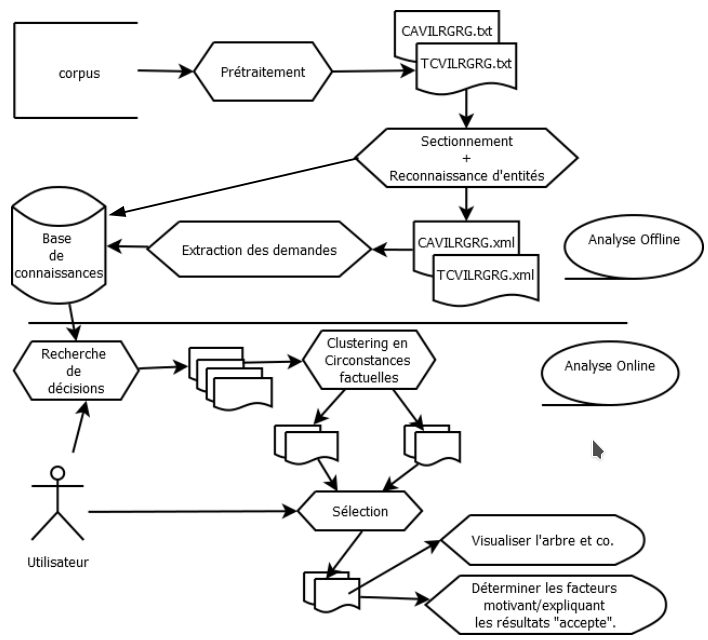
\includegraphics[width=0.8\textwidth]{pipelineComplet.png}

\end{frame}


%%-=-=-=-=-=-=-=-=-=-=-=-=-=-=-=-=-=-=-=-=-=-=-=-=
%%
%%	Questions
%%
%%-=-=-=-=-=-=-=-=-=-=-=-=-=-=-=-=-=-=-=-=-=-=-=-=
\section{Détection de sections et d'entités}


\begin{frame}{Sectionner les décisions pour organiser l'extraction}
\scriptsize
\begin{columns}
\begin{column}{.45\linewidth}
\fbox{\begin{minipage}{\textwidth}ARRÊT N°

R.G: \textcolor{red}{11/03924}

\textcolor{red}{COUR D'APPEL} DE \textcolor{red}{NÎMES}

\textcolor{red}{CHAMBRE CIVILE}

\textcolor{red}{1ère Chambre A}

ARRÊT DU \textcolor{red}{20 MARS 2012}

APPELANTE:

\textcolor{red}{Madame Michéle A.} ...

assistée de la \textcolor{red}{SELARL VAJOU}, ...

INTIMES:

\textcolor{red}{Monsieur Martial B} ...

assisté de la \textcolor{red}{SCP MARION GUIZARD PATRICIA SERVAIS}, ...

COMPOSITION DE LA COUR LORS DU DÉLIBÉRÉ:

\textcolor{red}{M. Dominique BRUZY, Président}

\textcolor{red}{M. Serge BERTHET, Conseiller}

...
\end{minipage}}
\vspace{0.1cm}

{\normalsize \textbf{Entêtes}: méta-données}
\end{column}
\begin{column}{.55\linewidth}
\fbox{\begin{minipage}{\textwidth}FAITS, PROCEDURE, ...

Madame Michèle A. demande:

...

- de condamner Madame JONES-B. à lui payer la somme de \textcolor{red}{2.500 euros} au titre de l'\textcolor{red}{article 700 du Code de Procédure Civile}, 
\end{minipage}}
\vspace{0.1cm}

{\normalsize \textbf{Corps}: demandes, arguments et normes }

\vspace{0.4cm}

\fbox{\begin{minipage}{\textwidth}PAR CES MOTIFS, LA COUR:

...

Vu l'\textcolor{red}{article 809 du Code de Procédure Civile},

...

\textcolor{red}{Déboute Madame A. de sa demande de provision sur dommages-intérêts.}

...

Vu l'\textcolor{red}{article 700 du Code de Procédure Civile},

Condamne Madame JONES-B. à verser à Madame A. la somme de \textcolor{red}{2.500 euros}.
\end{minipage}}
\vspace{0.1cm}

{\normalsize \textbf{Dispositif}: résultats et normes}

\end{column}
\end{columns}
\end{frame}

\begin{frame}{Entités et sections à détecter}

\scriptsize
\begin{table}[!htb]
\centering
%\scriptsize
\begin{tabular}[c]{|l|c|p{0.6\textwidth}|}
\hline
\textbf{Entités} & \textbf{Labels} & \textbf{Exemples}\\\hline
\multicolumn{3}{|c|}{\textbf{Section entête (E)}} \\
\hline
Numéro R.G. & \textbf{RG} & "10/02324", "60/JAF/09" \\ \hline
Ville & \textbf{VL}& "NÎMES", "Agen", "Toulouse" \\ \hline
Type de juridiction & \textbf{JR} & "COUR D'APPEL" \\ \hline
Formation & \textbf{FM} & "1re chambre", "Chambre économique" \\ \hline
Date & \textbf{DT} & "01 MARS 2012", "15/04/2014"\\ \hline
Partie appelante & \textbf{AP} & "SARL K.", "Syndicat ...", "Mme X ..."\\ \hline
Partie intimée & \textbf{IM} & - // - \\ \hline
Partie intervenante & \textbf{IV} & - // - \\ \hline
Avocat & \textbf{AV} & "Me Dominique A., avocat au barreau de Papeete"\\ \hline
Juge & \textbf{JG} & "Monsieur André R.", "Mme BOUSQUEL" \\ \hline
fonction du juge & \textbf{FT} & "Conseiller", "Président"\\ \hline
\multicolumn{3}{|c|}{\textbf{Corps (T) et dispositif (D)}} \\ \hline

Norme & \textbf{NO} & "l' article 700 NCPC", "articles 901 et 903"  \\ \hline
\hline
Élément à éviter & \textbf{O} & \textit{tout élément ne faisant partie d'aucune entité ciblée} \\ \hline
\end{tabular} 

\caption{Entités et leurs labels par section.}\label{relevantinfo}
\end{table}
\end{frame}

\begin{frame}{Architecture proposée}
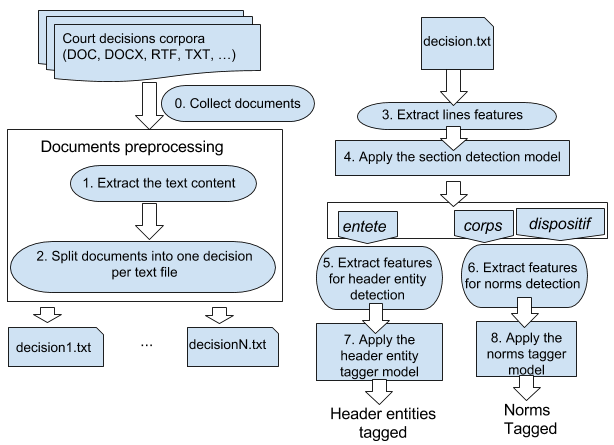
\includegraphics [width=\textwidth]{archAppli.png}
\end{frame}


\begin{frame}{Approches probabilistes d'étiquetage de séquence}
Modèles probabilistes à états et observations

\scriptsize
\begin{table}[]%width=\linewidth
	%\begin{tabular}[]{p{0.40\linewidth}|p{0.55\linewidth}}
	\begin{tabular}[]{c|c}
		\toprule
{\textbf{HMM}} & {\textbf{CRF}} \\
%		\midrule
%		\textbf{Generative} models 	& \multicolumn{2}{c}{"\textbf{Discriminative}" or "\textbf{Conditional}" models } \\[0.25em]
%\midrule		
%"\textbf{generate}" input	& {"\textbf{condition}" on input }\\%[0.25em]
\midrule
{un seul descripteur  par observation}	& {plusieurs descripteurs complexes par observation}\\%[0.25em]
\midrule	
		\begin{tikzpicture}[->,>=stealth',shorten >=1pt,auto,node distance=1.3cm,
                    semithick]
  \node[state] (S1)                    {$s_{t-1}$};
  \node[state]         (S2) [right of=S1] 	  {$s_{t}$};
  \node[state]         (O) [below of=S2] {$o_{t}$};
  \path (S1) edge              node {} (S2)
        (S2) edge              node {} (O);
\end{tikzpicture}
				& 

\begin{tikzpicture}[auto,>=stealth',shorten >=1pt,auto,node distance=1.3cm,
                    semithick]
  \node[state] (S1)                    {$s_{t-1}$};
  \node[state]         (S2) [right of=S1] 	  {$s_{t}$};
  \node[state]         (O) [below of=S2] {$o_{t}$};
  \path (S1) edge              node {} (S2)
        (S2) edge              node {} (O);
\end{tikzpicture}					
					\\%[0.25em]
\midrule
$P_\lambda(S,O) = \prod\limits_{t=1}^{T} P(s_t \vert s_{t-1}) * P(o_t \vert s_{t})$  & $P_\lambda(S|O) = \frac{1}{Z(O)}exp\left( \sum\limits_{t=1}^{T}\sum\limits_{k} \lambda_k f_k(s_{t-1},s_t, o_t) \right) $ \\
% & & & \\
\tiny \cite{Seymore1999hmm} & \tiny \cite{peng2006crf} \\ 
		\bottomrule
	\end{tabular}
\end{table}

\normalsize

Objectif: Trouver la séquence la plus probable d'étiquetage pour l'ensemble du texte

\textbf{Entrainement sur des textes manuellement annotés}
\end{frame}

\begin{frame}[c]{Premiers résultats \cite{tagny2017sectNerhmmcrf}}
\begin{table}[!htb]
\scriptsize

\centering
\begin{tabular}{|c|c|c|c|c|c|c|c|c|c|}
\hline
 & \multicolumn{3}{c|}{HMM}  & \multicolumn{3}{c|}{CRF-}  & \multicolumn{3}{c|}{CRF+} \\
\hline
\textit{labels} & P($\%$) & R($\%$) & F1 & P($\%$) & R($\%$) & F1 & P($\%$) & R($\%$) & F1 \\
\hline
 \multicolumn{10}{|c|}{\textit{\textit{Section Entête (E)}}} \\
\hline
 AP & 35.3 &  14.1 & 20.1  & 64.9 & 48.8 & 55.6 & 92.0 & 86.7 & 89.3 \\
\hline
 AV & 83.8 &  98.3 & 90.5  & 96.4 & 97.5 & 96.9 & 97.6 & 98.1 & 97.9 \\
 \hline
 DT & 70.9 & 72.6 & 71.7  & 94.4 & 86.8 & 90.4 & 98.8 & 97.7 & 98.2 \\
 \hline
FM & 87.6 &  93.7 & 90.5  & 98.8 & 98.4 & 98.6 & 98.9 & 99.3 & 99.1 \\
 \hline
FT &  88.8 & 59.8 & 71.3  & 94.2 & 92.3 & 93.3 & 97.1 & 95.5 & 96.3 \\
 \hline
IM  & 53.1 & 57.4 & 55.1  & 67.2 & 64.6 & 65.8 &  89.3 & 88.1 & 88.7  \\
 \hline
 \textcolor{red}{IV} & - & 2.2 & - & 25.9 & 26.5 & 26.2 & 67.3 & 41.4 & \textcolor{red}{46.4} \\
 \hline
JG  & 68.0 & 85.7 & 75.7  & 96.2 & 95.7 & 96.0 & 98.1 & 97.7 & 97.9 \\
 \hline
JR  & 75.8 & 99.5 & 86.0  & 98.6 & 99.4 & 99.0 & 99.3 & 99.4 & 99.4 \\
 \hline
RG  &  - & 0  & - & 83.7 & 46.1 & 59.4 & 98.6 & 97.4 & 98.0 \\
\hline
VL & 93.1 & 27.9 & 42.6  & 98.2 & 98.4 & 98.3 & 99.0 & 99.0 & 99.0 \\
\hline
 \multicolumn{10}{|c|}{\textit{\textit{Sections inférieures (T \& D )}}} \\
 \hline
NO & 92.9 & 90.9 & 91.9 & 96.0 & 93.8 & 94.9 & 97.9 & 96.5 & 97.2\\
\hline
\end{tabular}

 \textit{5-fold validation croisée avec 500 documents annotées manuellement}
\caption{Précision (P), rappel (R), F1-mesure (F1) au niveau des mots.}\label{prf-entity}
\end{table}
\end{frame}

\section{Extraction d'informations sur les demandes}

\begin{frame}{Extraction des informations sur les demandes}
\begin{table}
\centering 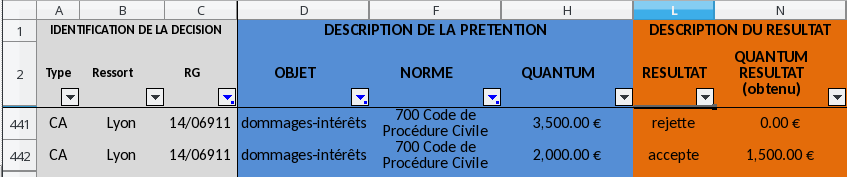
\includegraphics[width=\textwidth]{tab-annotations-dmd.png}
\caption{\scriptsize Tableau des informations sur les demandes}
\end{table}

\begin{block}{Exemple: Informations pertinentes à extraire}%CAANG1500238.xml
\begin{itemize}\scriptsize
%\item \textbf{Position de la partie}: Intimé
\item \textbf{Catégorie prédéfinie}: Dommages-intérêts pour procédure abusive
\begin{itemize}\scriptsize
\item \textbf{Objet}: Dommages-intérêts
\item \textbf{Fondement}: Articles 1382 code civil et 32-1 code de procédure civile
\end{itemize}
\item \textbf{Quantum demandé}: 20 000 euros
\item \textbf{Sens du résultat} : "\textit{rejette}"
\item \textbf{Quantum accordé} : 0 euros
\end{itemize}
\end{block}
\end{frame}

\begin{frame}{Difficultés (1)}
%\small
Expressions non structurées, par  \textcolor{orange}{référence}, par \textcolor{blue}{agrégation}

\begin{exampleblock}{Exemple (suite): Expression de demande} % CAANG1500238.xml
La société A. conclut à la confirmation du jugement entrepris sauf à
former appel incident sur la disposition du jugement l'ayant déboutée de sa
demande de \textbf{dommages intérêts pour abus de procédure} et elle demande à la cour de
condamner l'appelante à lui payer la somme de \textbf{20 000 euros} à titre de dommages
intérêts ...

\end{exampleblock}

\begin{exampleblock}{Exemple (suite): Expression de resultat}
La cour, ... 

Confirme \textcolor{orange}{la décision entreprise} en \textcolor{blue}{toutes ses dispositions},
\end{exampleblock}
\end{frame}

\begin{frame}{Difficultés (2)}
\begin{alertblock}{}
\begin{itemize}
\item Présence de plusieurs demandes de catégories similaires et/ou différentes dans une m\^eme décision
\item Toutes les catégories ne sont pas connues d'avance
\end{itemize}
\end{alertblock}
\end{frame}

\begin{frame}{Proposition: Extraction des demandes par catégorie}


\centering 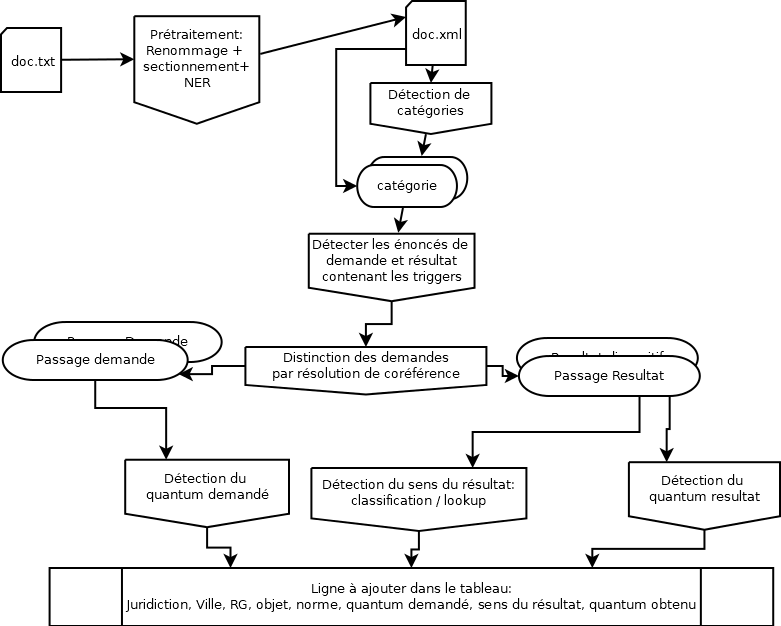
\includegraphics[width=0.8\textwidth]{pipeline-dmd.png}

{\scriptsize
\begin{itemize}
\item Méthode générique qui s'adapte aux spécificités de la catégorie traitée
\item Définition incrémentale des catégories
\end{itemize}
}
\end{frame}


\begin{frame}{Apprentissage des termes caractéristiques des catégories}
\begin{table}[!htb]
\begin{center} \scriptsize
\begin{tabular}{|l||p{0.16\textwidth}|p{0.16\textwidth}|p{0.16\textwidth}|p{0.16\textwidth}|}
\hline
Catégories & \multicolumn{4}{c|}{Termes} \\ \hline
\textit{acpa} & amende civile & 32-1 du code & amende & article 32-1 \\ \hline 
 \textit{concdel} & actes de concurrence & désorganisation & concurrence déloyale & salarié démissionnaire   \\ \hline
 \textit{danais} & procédure abusive & abus & abusive & 32-1   \\ \hline
 \textit{dcppc} & créance déclarée & juge-commissaire & 
chirographaire & admet la créance  \\ \hline
  \textit{doris} & trouble anormal & anormal & voisinage & trouble  \\ \hline
 \textit{styx} & 700 du code & article 700 & 700 & lieu à application  \\ \hline

\end{tabular}
\end{center}
\caption{premiers termes pour chaque catégorie (de gauche à droite)}\label{termes-select}
\end{table}
$ngl(w,c) = \frac{\sqrt{N} ((N_{w,c} N_{\overline{w},\overline{c}}) - (N_{w,\overline{c}} N_{\overline{w},c}))}{\sqrt{N_w N_{\overline{w}} N_c N_{\overline{c}}}}$ \cite{ng1997ngl}
\end{frame}


\begin{frame}{Evaluation de l'extraction de demande-résultat}
\scriptsize
$\forall D_j \in D_+ = \lbrace D_1, D_2, ..., D_{\vert D_+ \vert} \rbrace$ 

avec $D_+$ : l'ensemble des documents annotés et contenant la catégorie
\[Precision_{I_s,j} = \frac{\# {I_s} \text{ bien identifiées dans } D_j}{\# {I_s} \text{ identifiées dans } D_j}  = \frac{TP_{I_s,j}}{{TP_{I_s,j} + FP_{I_s,j}}} \]

\[Rappel_{I_s,j} = \frac{\# I_s \text{ bien identifiées dans } D_j}{\#  I_s \text{ dans la vérité terrain de } D_j} =  \frac{TP_{I_s,j}}{{TP_{I_s,j} + FN_{I_s,j}}}\]

avec  $\#I_s$ = nombre de tuples d'informations dont le type appartient à $I_s$

\[Precision_{I_s} = \frac{\sum\limits^{\vert D_+ \vert}_{j=1}{Precision_{I_s,j}}}{\vert D_+ \vert} \text{\hspace{3cm}} Rappel_{I_s} = \frac{\sum\limits^{\vert D_+ \vert}_{j=1} Rappel_{I_s,j}}{\vert D_+ \vert}\]

\[F1_{I_s} =2 \times \frac{Precision_{I_s} \times Rappel_{I_s}}{Precision_{I_s} + Rappel_{I_s}}\]
\end{frame}

\begin{frame}{Résultats actuels de l'extraction de demande-résultat}
\begin{center}
\tiny
\begin{tabular}{|c||c||c|c|c|c||c|c|c|c|}
\hline
Catég. & $I_s$ & \multicolumn{4}{c||}{Train} & \multicolumn{4}{c|}{Test} \\ \hline
 & &  P & R & F1 & Doc & P & R & F1 & Doc  \\ \hline
 \multirow{3}{*}{acpa} & Q-DMD & 0.607 & 0.643 & 0.624 & 0.571 & 0.611 & 0.667 & 0.638 & 0.556  \\
 & SENS RST & \textcolor{blue}{0.964} & \textcolor{blue}{1.0} & \textcolor{blue}{0.982} & \textcolor{blue}{0.929} & 0.833 & \textcolor{blue}{0.889} & \textcolor{blue}{0.86} & 0.778  \\
 & Q-RST & \textcolor{blue}{0.964} & \textcolor{blue}{1.0} & \textcolor{blue}{0.982} & \textcolor{blue}{0.929}  & 0.833 & \textcolor{blue}{0.889} & \textcolor{blue}{0.86} & 0.778   \\\hline
\multirow{3}{*}{concdel} & Q-DMD & \textcolor{red}{0.361} & \textcolor{red}{0.4} & \textcolor{red}{0.38} & \textcolor{red}{0.333} & \textcolor{red}{0.167} & \textcolor{red}{0.167} & \textcolor{red}{0.167} & \textcolor{red}{0.167} \\
 & SENS RST & 0.833 & 0.596 & 0.695 & \textcolor{red}{0.444} & 0.819 & 0.715 & 0.764 & \textcolor{red}{0.417}  \\
 & Q-RST & 0.843 & 0.651 & 0.735 & \textcolor{red}{0.444} & 0.819 & 0.715 & 0.764 & \textcolor{red}{0.417}   \\ \hline
\multirow{3}{*}{danais} & Q-DMD & \textcolor{red}{0.312} & \textcolor{red}{0.343} & \textcolor{red}{0.327} & \textcolor{red}{0.271}  & \textcolor{red}{0.38} & \textcolor{red}{0.392} & \textcolor{red}{0.386} & \textcolor{red}{0.367} \\
 & SENS RST & \textcolor{blue}{0.88} & \textcolor{blue}{0.922} & \textcolor{blue}{0.901} & 0.797 &  \textcolor{blue}{0.905} & \textcolor{blue}{0.911} & \textcolor{blue}{0.908} & \textcolor{blue}{0.861} \\
 & Q-RST & \textcolor{blue}{0.901} & \textcolor{blue}{0.938} & \textcolor{blue}{0.919} & 0.805 & \textcolor{blue}{0.918} & \textcolor{blue}{0.924} & \textcolor{blue}{0.921} & \textcolor{blue}{0.873} \\ \hline
 \multirow{3}{*}{dcppc} & Q-DMD & \textcolor{red}{0.078} & \textcolor{red}{0.078} & \textcolor{red}{0.078} & \textcolor{red}{0.078} &  \textcolor{red}{0.059} & \textcolor{red}{0.059} & \textcolor{red}{0.059} & \textcolor{red}{0.059}  \\
 & SENS RST & \textcolor{blue}{0.961} & \textcolor{blue}{0.873} & \textcolor{blue}{0.915} & 0.824 &  \textcolor{blue}{0.912} & 0.797 & \textcolor{blue}{0.85} & 0.735  \\
 & Q-RST & 0.775 & 0.711 & 0.741 & 0.667 &  0.765 & 0.65 & 0.702 & 0.588 \\ \hline
\multirow{3}{*}{doris} & Q-DMD & \textcolor{red}{0.105} & \textcolor{red}{0.083} & \textcolor{red}{0.093} & \textcolor{red}{0.079} & \textcolor{red}{0.18} & \textcolor{red}{0.148} & \textcolor{red}{0.162}  & \textcolor{red}{0.08}  \\
 & SENS RST & 0.553 & \textcolor{red}{0.456} & \textcolor{red}{0.5} & \textcolor{red}{0.368} & 0.5 & \textcolor{red}{0.385} & \textcolor{red}{0.435} & \textcolor{red}{0.28}   \\
 & Q-RST & 0.579 & \textcolor{red}{0.482} & 0.526 & \textcolor{red}{0.395} & 0.54 & \textcolor{red}{0.395} & \textcolor{red}{0.456} & \textcolor{red}{0.28}   \\ \hline
\multirow{3}{*}{styx} & Q-DMD & 0.733 & 0.633 & 0.68 & 0.533 & 0.575 & 0.525 & 0.549 & \textcolor{red}{0.4}  \\
 & SENS RST & \textcolor{blue}{0.983} & 0.783 & \textcolor{blue}{0.872} & 0.567 & 0.825 & 0.642 & 0.722 & \textcolor{red}{0.35} \\
 & Q-RST & \textcolor{blue}{0.983} & 0.783 & \textcolor{blue}{0.872} & 0.567 &   \textcolor{blue}{0.85} & 0.642 & 0.731 & \textcolor{red}{0.35}  \\ \hline
\end{tabular} 
\end{center}
\tiny

$I_s \subset I = \lbrace \text{Q-DMD, SENS RST, Q-RST} \rbrace$

\textit{P, R, F1 = resp. $Precision_{I_s}, Rappel_{I_s}, F1_{I_s}$}

\textit{Doc = proportion de documents dans lesquels toutes les infos ont été bien identifiées}

Code couleur: \textcolor{blue}{bleu}: mesure >= 0.85;  \textcolor{red}{rouge}: mesure < 0.5
\end{frame}

\section{Conclusion}

\begin{frame}{Résumé des résultats actuels}
\begin{itemize}
\item Bons résultats pour la détection d'entités et de sections à base de CRF
\begin{itemize}
\item Difficultés:
\begin{itemize}
\item Annotation manuelle d'un jeu suffisant d'exemples
\item Identification de bons descripteurs 
\end{itemize}
\item Limite de l'approche:
\begin{itemize}
\item Descripteurs définis manuellement 
\item Etiquetage en plusieurs passes 
\end{itemize}
\end{itemize}
\item Premiers résultats encourageants sur l'extraction de demande par catégorie:
\begin{itemize}
\item Identification facile de la présence d'une catégorie par classification binaire
\item Le sens et le quantum résultat semblent facile à identifier 
\item Difficultés: identification des termes-clés d'expression des demandes et résultats
\end{itemize}
\end{itemize}

\end{frame}

\begin{frame}{Résumé des t\^aches du projet}

\begin{enumerate}
\setlength\itemsep{1.5em}
\item Extraction d'information: métadonnées, demande-résultat, situations factuelles d'une catégorie de demande (par ex. \textit{licenciement} ou \textit{divorce})
\item Standardisation et représentation des informations extraites sous forme de base de connaissances
\item Détermination des facteurs associables aux décisions des juges 
\end{enumerate}

\end{frame}

\section{Questions?}

%\begin{frame}{Quelle aide à l' \og analyse \fg{} est précisément attendue?}
%\begin{enumerate}
%\setlength\itemsep{2em}
%\item Comparaison des taux des types de résultat : 
%
%positif vs. négatif ...
%\begin{itemize}
%\setlength\itemsep{1em}
%\item pour une catégorie définie de demandes
%\item dans une situation factuelle d'intérêt
%\end{itemize}
%\item Détermination d'idées associées à un type de résultat 
%\begin{itemize}
%\setlength\itemsep{1em}
%\item faits
%\item arguments
%\end{itemize}
%\end{enumerate}
%\end{frame}
%
%\begin{frame}{Organisation prévisionnelle de la rédaction}
%\begin{enumerate}
%\item Introduction (Positionnement, Attendu, défis, généralités sur les compétences techniques nécessaires)
%\item Étude bibliographique: Analyse sémantique et prédictive des décisions judiciaires
%\item Extraction/détection d'information à partir de texte: expression et résolution d'entités, de demandes et de résultats, liaison des demandes et résultats correspondances
%\item Interprétation: Catégorisation des demandes et résultats
%\item Explication : détermination des facteurs liés au sens du résultat
%\item Conclusion: apport, voies d'amélioration, autres problématiques  
%\end{enumerate}
%\end{frame}

%-=-=-=-=-=-=-=-=-=-=-=-=-=-=-=-=-=-=-=-=-=-=-=-=
%	References:
%-=-=-=-=-=-=-=-=-=-=-=-=-=-=-=-=-=-=-=-=-=-=-=-=
\begin{frame}[t,allowframebreaks]{References}
\tiny
\bibliographystyle{apalike}
\bibliography{references}	
\end{frame}

\end{document}
